% Chapter 5

\chapter{CA Guide Back End} % Main chapter title

\label{backend} % For referencing the chapter elsewhere, use \ref{Chapter1} 

\lhead{Chapter 5. \emph{CA Guide Back End}} % This is for the header on each page - perhaps a shortened title

%----------------------------------------------------------------------------------------

\section{Introduction}

The CA Guide back end is meant to be used by the park or museum staff responsible for designing and optimizing the visiting experience. In contrast to the front end, the user interface can be more complex requiring an introductory training and support. Of course, the usability deserves special attention in spite of the training, as it has a major influence on the frequency a software is used, the attitude towards it and so the success of the whole product. %TODO Citation

There are two main tasks accomplished with the CA Guide back end:

\begin{itemize}
\item Modeling the outdoor or indoor site by defining areas on a map or floor plan and adding content that later will be presented on the mobile device when entering this area. Especially for indoor sites, single Bluetooth beacons with their identifying numbers and positions must be added to the plan to enable the mobile device to locate itself.
\item Analytic functions for understanding how the visitors move trough the exhibition and thus allowing to optimize it, similar to the way the behavior of website visitors is tracked and used to optimize the web presence\footnote{Of course, the privacy of the visitor has to be respected at any time. The data must only be collected anonymously and with the permission of the visitor.}.
\end{itemize}

%TODO Mockups
%TODO In Place editing

\section{The Target Platform}

The back end user interface has to run in a standard web browser without specific plugins. This has several advantages: Users can start immediately to work with the product without installing any client. Having the project data in a cloud database, they can work on the same project from different locations using different computers without manually setting up a synchronization infrastructure. Computation expensive analytic functions can be performed directly on the database or web/application servers and only the results are transferred to the client, enabling it's usage on common hardware.

By allowing collaborative editing, the museum staff can easily be supported remotely in real time without having to be on site. 

\section{Architectural Decisions}

\subsection{The Client and Server Code Gap}
One of the main challenges developing for the web is the client/server code barrier. 

Modern web applications need to be highly responsive for providing a good user experience and thus be accepted by them. Operations like adding, editing or deleting entities have to be performed without having to do a full page reload to display some sort of HTML form and reloading the whole page again after the form was submitted to the server. This can be achieved using asynchronous calls to the server in the background, exchanging only the needed data with the server and refreshing just the needed part of the HTML DOM. Many operations like resorting a table can even be performed completely in the browser without even performing a server request.

This technique is commonly known as AJAX (Asynchronuous JavaScript and XML) and inside this acronym's phrase one can already spot the main problem. While AJAX gained popularity during the last years, it leveraged the massive use of JavaScript, a dynamically typed scripting language originally not designed for big projects. In fact, JavaScript was developed in 1995 by Brendan Eich in ten days for the Netscape browser, which is an extremely short time despite Eich's big experience in building languages \cite{interview-eich}. That led him to design the language to be malleable, and there are many libraries making programming in JavaScript a little less painful, without solving the problem of lacking static types.

So the two main problems to be solved are:

\begin{itemize}
\item Some data structures and algorithms already existing in the server code have to reprogrammed for the client running in the browser, creating redundancy with all the known problems it has
\item The standard programming language for client-side code lacks static typing and a class syntax, among others
\end{itemize}

The next subsection focuses on different solution attempts.

\subsection{Solution Attempts}

\subsubsection*{Improved Javascript}

In the last years, several new scripting languages are emerging that compile to JavaScript. 

One of this languages was even integrated in the Play framework, which comes with an built in compiler for CoffeeScript \cite{coffeescript}. It is a small language that provides a nicer syntax for JavaScript, introducing even classes and inheritance, and compiles to plain JavaScript. However, it does not add any support for static typing.

Another noteworthy web-client language is TypeScript, which is maintained by Microsoft as open source \cite{typescript}. As the name implies, it adds static typing to JavaScript with type inference and similar to CoffeeScript it enhances the syntax. In contrast to CoffeeScript, it is a superset of JavaScript, meaning any JavaScript code is automatically valid TypeScript code, too. 
For using third party libraries in a typed way, a big repository with open source type definitions for 796 libraries at the time of writing \cite{typescript-repo}. By including a reference to such a type definition, the library's API can be accessed in a statically typed way.

This screenshot demonstrates a TypeScript compilation error and an inferred numeric type.
\begin{figure}[H]
\centering
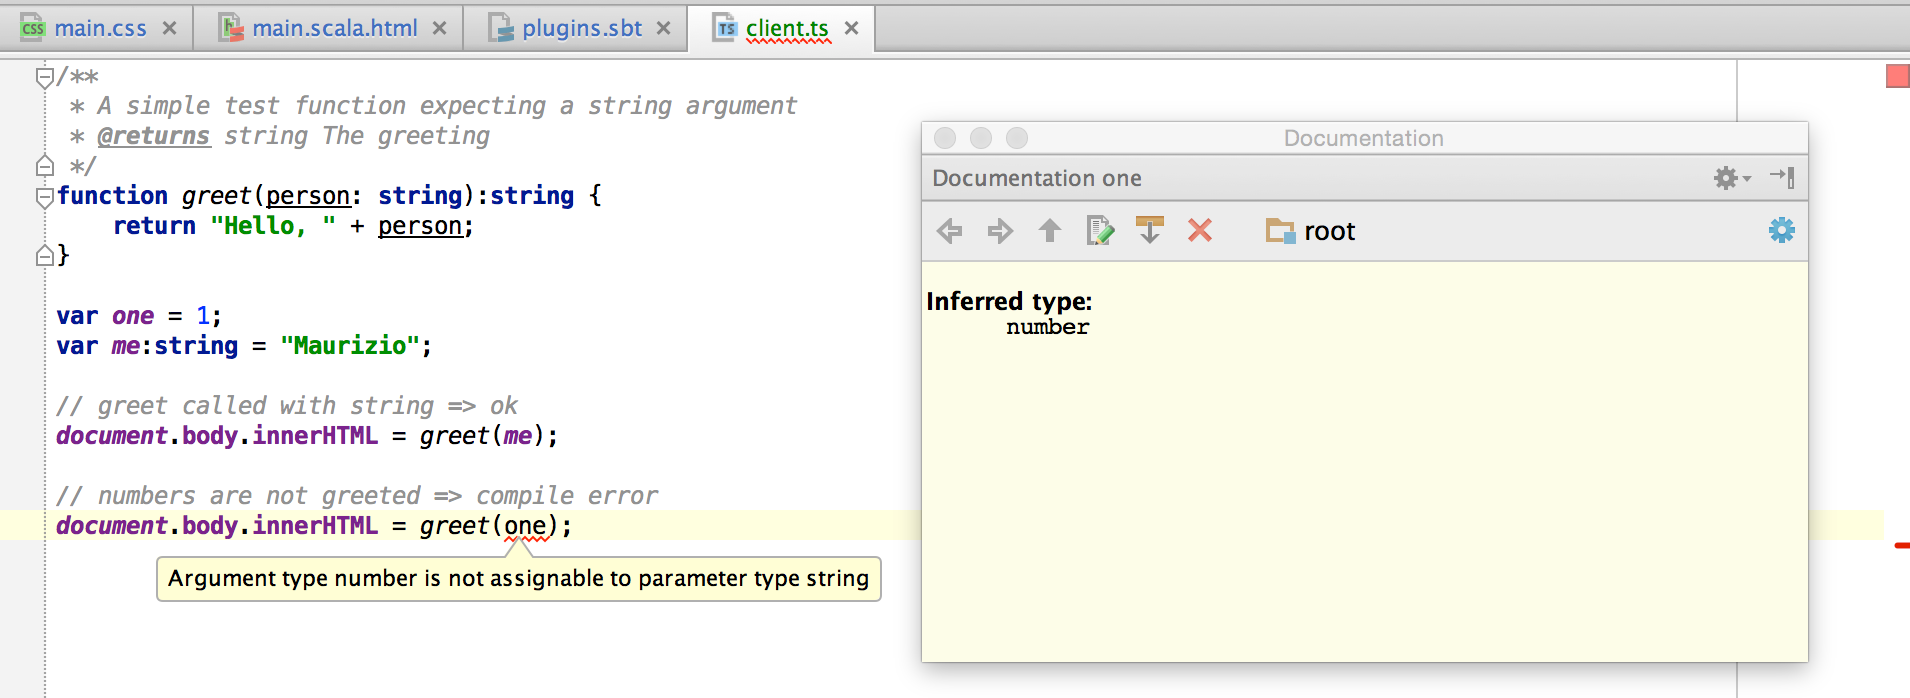
\includegraphics[width=0.9\textwidth]{typescript-idea.png}
\caption{TypeScript in IntelliJ IDEA}
\end{figure}

While these solutions, and especially TypeScript, smooth out the main flaws of JavaScript and are being adopted by a rising number of developers, they do not solve the need to create redundancy in client/server web applications. So for this work, I continued to search for a solution to both problems.

\subsubsection*{Unified Programming Language for Server and Client Code}

There are several attempts to bring JavaScript on the server, and the most popular is Node.js, which was released in 2009. While there surely are some scenarios for server-side JavaScript like screen-capturing of rendered websites, in my opinion this is the wrong way of language unification. It brings the problems connected to JavaScript to the server side, where much better designed languages exist, like Scala. 

The other way around would be the perfect solution: Using a rich and well engineered language to write server and client code. So after some research I found the Scala.js project \cite{scalajs}. It was started on February 2013 by Sébastien Doeraene, a member of the Scala team at LAMP (Programming Methods Laboratory at EPFL), after Martin Odersky suggested him to work on a JavaScript compiler \cite{scalajs-interview}.

%TODO most Scala features 
%TODO cross compiling

On 5th February 2015, at the time of this writing and exactly two years after this project was started, the release v0.6.0 was announced on the official Scala website and the experimental flag was removed, defining Scala.js "production-ready" \cite{scalajs06}.

So I decided to try this very promising compiler for the Guide back end client-side code.

\section{Setting up the Development Platform}

\subsection{Scala and Play}

Scala is used as programming language for the back end, with Play web framework as a basis for developing a web application in Scala.

%less as css

\subsection{Adding Reactive Couchbase as Scala Database Driver}

%build.sbt
%connecting to couchbase database server (conf/applicatin.conf)
%conf/play.plugins

\subsection{Adding Scala.js for Web Client Code}

%Motivation for Typescript

\subsection{Adding Bootstrap as UI Framework}


\section{Architecture}

\subsection{Overview}

%Single page,  

\subsection{The REST HTTP Interface}

%HTTP methods
%Excerp routing file, reverse routing, single place of definition

\subsection{Performing Database Queries using Scala Futures}

The interface of the Reactive Couchbase Driver makes extensive use of Futures, a language feature introduced in Scala 2.10\footnote{The most recent Edition of \cite{scala-book} at the time of writing doesn't cover Scala 2.10. A more detailed description of Futures can be found in the Scala Online Documentation \cite{scala-futures}.}.

In this section the Future concept is explained using a simple query which retrieves a list of all sites stored in the guide-editor Couchbase bucket.









